%*******************************************************************************
% Copyright (c) 2014 Formal Mind GmbH and others
% All rights reserved. This program and the accompanying materials
% are made available under the terms of the Eclipse Public License v1.0
% which accompanies this distribution, and is available at
% http://www.eclipse.org/legal/epl-v10.html
% 
% Contributors:
%     Michael Jastram - initial Copy
%     Maha Jastram - susequent improvements
%******************************************************************************/

% ===================================================================================
\section{Acknowledgements}
% ===================================================================================

Many parties were involved in the creation of RMF.  We would like to thank the core team that made it possible.

\begin{figure}
  \centering
  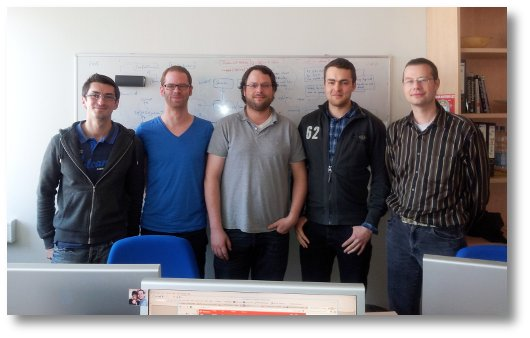
\includegraphics[width=\textwidth]{../rmf-images/2012_03_sprint_team.jpg}
  \caption{The RMF team during a Sprint in April 2012 in Düsseldorf, Germany: Lukas Ladenberger, Mark Brörkens, Ingo Weigelt, Said Salem and Michael Jastram (left to right)}
  \label{fig:intro_core_team}
\end{figure}

The roots of this project were created by Andreas Graf, Michael Jastram and Nirmal Sasidharan, who joined together individual projects to create RMF.  Their efforts were financed by the research projects itea Verde and FP7 Deploy.  RMF was assembled at the Eclipse Foundation, where it has been active ever since.  Figure~\ref{fig:intro_core_team} shows four of the five RMF Committers at a joint coding session (missing is Andreas Graf).

